% ------------------------------------------------------------------------------ %

  \documentclass[a4paper,11pt]{report}

% ------------------------------------------------------------------------------- %
%LANGUAGE PACKS%

  \usepackage[english]{babel} 
 % ------------------------------------------------------------------------------- %
%FONTS%    
  \usepackage[utf8x]{inputenc}
  
  \usepackage{amsmath}
  \usepackage{multirow}
  \usepackage{enumerate}
  \usepackage{verbatim}
  \usepackage{listings}
% ------------------------------------------------------------------------------- %
%LAYOUT%  

\usepackage{fullpage}

 \tolerance=1
 \emergencystretch=\maxdimen
 \hyphenpenalty=10000
 \hbadness=10000
 \newcommand{\HRule}{\rule{\linewidth}{0.5mm}}
 
 \usepackage[pdftex]{graphicx} 

 
 \usepackage{hyperref}

 \hypersetup{
    colorlinks,
    citecolor=black,
    filecolor=black,
    linkcolor=black,
    urlcolor=black
}
\lstset {breaklines=true,
extendedchars=false,
showstringspaces=false}

% ------------------------------------------------------------------------------- %

% ------------------------------------------------------------------------------- %


\begin{document}

\begin{titlepage}

\begin{center}


\includegraphics{images/UvA-logo-2a.png}~\\[1cm]

\textsc{\LARGE System and Network Engineering\\ OS3 Group}\\[1.5cm]

\HRule \\

{ \huge \bfseries Essential Skills\\Latex Assignment}

\HRule \\[1cm]

\large{Diana Rusu} \\
\large{Alexandros Stavroulakis}\\
\large{Nikolaos Petros Triantafylldis}\\[11cm]

\today
\end{center}
\end{titlepage}

\tableofcontents

\listoffigures

\listoftables

\chapter* {Introduction}
\addcontentsline{toc}{chapter}{Introduction}

This is our report for Latex assignment for the Essential Skills module. This report was written collaboratively via a public git repository hosted in github.com. All conflicts were resolved with loads of love. \\[0.5 cm]
\emph{Diana Rusu}\\
\emph{Alex Stavroulakis}\\
\emph{Nick Triantafyllidis}\\


\chapter{XML in the Semantic web : RDF}

\section{Semantic Web}

\paragraph{}Semantic Web is a framework for sharing data between applications, enterprises and people, independent of platform and software(W3C).

Semantic refers to  {\color{red}meaning}. It is "a web of data that can be processed directly and indirectly by machines" - Tim Berners Lee

Extends the internet which comprises web-pages readable only to humans, to websites that use metadata and can be read by machines.

This leads to the creation of "smart" services that can perform tasks for users with better results and help them share and fin info more easier.

Example : A human can utilize the web to search, find, compare and choose the lowest price to a product. Machines cannot since the webpages aren't build to be read by them.

Semantic Web is a form of information that can be interpreted by machines so they can accomplish the tedious tasks that contain searching, putting together and editing what's already available online.

\paragraph{}

\begin{figure}[h]
	\centering
		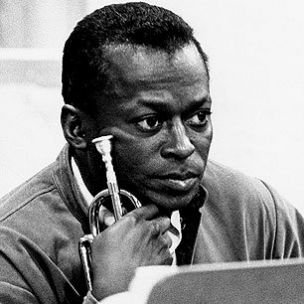
\includegraphics[width=90mm]{images/semantic-web-3.jpg}~\\[1cm]
		\caption {Example of triple \url {http://computer.howstuffworks.com/semantic-web3.htm}}
\end{figure}

 A URI gives a computer a specific point of reference for each item in the triple (subject,property and object) -- there is no need or interpretation or potential for misunderstanding.

\section{RDF}
\paragraph{}
RDF short for Resource Description Framework language is a  {\color{red}cross-platform framework} for describing resources on the web.It is written in XML and it's a W3C Recommendation.

As we can see in Fig1. RDF format consists of triple relationship: a subject, a predicate(property), and an object. RDF is the foundation upon which the web semantic data is build.

XML-based RDF allows a common way to describe and share information between different types of applications operating systems and computers.
 

\subsection{RDF Example}
\paragraph{}
The following example will give a more idea on how RDF works. \cite{w3schools}
 \paragraph{}
Here are two records from a CD-list:
 
\begin{table}[h]
\centering
\begin{tabular}{ | l | c | c | c | c | c |}
 \hline
 Title & Artist & Country & Company & Price & Year \\ \hline
 Empire Burlesque & Bob Dylan & USA &	Columbia & 10.90 &	1985 \\
 \hline
  Hide your heart & Bonnie Tyler & UK &	CBS Records &9.90 &	1988 \\
 \hline
\end{tabular}
\caption[A list of Albums]{A list of Albums}
\end{table}

\paragraph{}
Below a few lines from an RDF document:

\begin{lstlisting}[language=XML]
<?xml version="1.0"?>
<rdf:RDF
xmlns:rdf="http://www.w3.org/1999/02/22-rdf-syntax-ns#"
xmlns:cd="http://www.recshop.fake/cd#">

<rdf:Description
rdf:about="http://www.recshop.fake/cd/Empire Burlesque">
  <cd:artist>Bob Dylan</cd:artist>
  <cd:country>USA</cd:country>
  <cd:company>Columbia</cd:company>
  <cd:price>10.90</cd:price>
  <cd:year>1985</cd:year>
</rdf:Description>

<rdf:Description
rdf:about="http://www.recshop.fake/cd/Hide your heart">
  <cd:artist>Bonnie Tyler</cd:artist>
  <cd:country>UK</cd:country>
  <cd:company>CBS Records</cd:company>
  <cd:price>9.90</cd:price>
  <cd:year>1988</cd:year>
</rdf:Description>
.
.
.
</rdf:RDF> 


\end{lstlisting}
\paragraph{}
The first line of the RDF document is the XML declaration. The XML declaration is followed by the root element of RDF documents: \textbf{\textless rdf:RDF\textgreater}.

The xmlns:rdf namespace, specifies that elements with the rdf prefix are from the namespace "http://www.w3.org/1999/02/22-rdf-syntax-ns\#".

The xmlns:cd namespace, specifies that elements with the cd prefix are from the namespace "http://www.recshop.fake/cd\#".

The \textless rdf:Description\textgreater element contains the description of the resource identified by the rdf:about attribute.

The elements: \textbf{\textless cd:artist\textgreater}, \textbf{\textless cd:country\textgreater}, \textbf{\textless cd:company}\textgreater, etc. are properties of the resource.

\section{References}
\paragraph{}
Slide presentation for this topic can be found on the following link : \url{https://docs.google.com/file/d/0BzZaPwl3dLnFeW0tZGV5bHdRNUU/edit?usp=docslist_api} \cite{w3crdf,rdfrules,wikirdf,semantic,video1}

\chapter{XQuery}

\begin{figure}[h]
	\centering
		
\includegraphics{images/xquery_image.jpeg}~\\[1cm]
		\caption {XQuery}
\end{figure}

\section{Definiton}


\paragraph{}
\textbf{Xquery} is to XML formatted data what SQL is to relational databases. \cite{wikixquery}

\begin{itemize}
  \item \textbf{Xquery} is a specification from \textit{W3C}, appeared in 2007 and became a \textit{W3C} reccomendation. \cite{w3xquery}
  \item Current version 3.0.
  \item It is a language that uses queries to extract data from XML file or XML-like files.
  \item It contains a superset of Xpath expression syntax. \cite{xpath}
\end{itemize}
 
 Also, \\
 
 \begin{enumerate}
  \item \textbf{XQuery} is extensible.
  \item It contains many functions such as mathematical operations.
  \item If a function is needed and is not found, it can be added or programmed.
  \item Vendor-specific extensions allow other formats than XML to be queried.
\end{enumerate}


\paragraph{}
This presentation was a \emph{collaboration} between these groups: \\
 
\begin{table}[h]
\centering
 \begin{tabular}{| l | c | c | c |}
 \hline \textbf{Group} & \textbf{Student} & \textbf{Link} \\
 \hline 
 4 & Alex Stavroulakis & \href{https://www.os3.nl/2014-2015/students/alexandros_stavroulakis/es}{Wiki}\\
 \hline 
 5 & Guido Kroon & \href{https://www.os3.nl/2014-2015/students/guido_kroon/es/assignments1}{Wiki} \\ 
 \hline 
 6 & Rophrimardho & \href{https://www.os3.nl/2014-2015/students/rohprimardho/es/homework_1.3}{Wiki} \\ 
 \hline 
 \end{tabular} 
 \caption[Collaboration Table]{Collaboration Table}
\end{table}
 


\chapter{RegEx Text Directed Engine}

\begin{figure}[h]
	\centering
		
\includegraphics{images/regexp_logo.png}~\\[1cm]
		\caption{Regular Expressions}
\end{figure}

\section{Types of Engines}
\begin{flushleft}
Two basic engine types reflect a fundamental difference in algorithms available for applying a regular expression to a string. The \textbf{NFA}(Non Deterministic Finite Automations) "regex-directed" engines and the \textbf{DFA} (Deterministic Finite Automations) "text-directed" engines. \cite{NFA,DFA}
\end{flushleft}

\section{Text-directed Engines}
\begin{center}
According to Jeffrey E. F. Friedl’s book "Mastering Regular Expressions" a DFA engine, each character scanned from the text controls the engine. \cite{book}
\end{center}

\section{How does it Work}
\begin{flushright}
It walks through the input string attempting all permutations of the regular expression before reading the next character in the string. It does not use backtracking
\end{flushright}

\section{Where is it used}
\begin{itemize}
  \item egrep
  \item awk
  \item MySQL etc\ldots
\end{itemize}

\paragraph{}
This presentation was a \emph{collaboration} between these groups: \\

\begin{table}[h]
\centering
 \begin{tabular}{| l | c | c | c |}
 \hline \textbf{Group} & \textbf{Student} & \textbf{Link} \\
 \hline 
 4 & Alex Stavroulakis & \href{https://www.os3.nl/2014-2015/students/alexandros_stavroulakis/es}{Wiki}\\
 \hline 
 5 & Dragos Barosan & \href{https://www.os3.nl/2014-2015/students/dragos_barosan/es/week2#homework_3}{Wiki} \\ 
 \hline 
 6 & Carlo Rengo & \href{https://www.os3.nl/2014-2015/students/carlo_rengo/es/homewrk_3}{Wiki} \\ 
 \hline 
 \end{tabular} 
 \caption[Collaboration Table]{Collaboration Table}
\end{table}

\chapter {Build Tools: Scons}

\begin{figure}[h]
	\centering
		
\includegraphics{images/scons-logo-transparent.png}~\\[1cm]
		\caption{Scons Build Tool}
\end{figure}

\section{What is SCons}

\paragraph{}

SCons is an open source software construction tool written in Python. It defines itself as a next-generation build tool and it is intended as a replacement of tools such as CMake and GNU autotools. 

\section{Why is SCons used}

\paragraph{}

SCons prides it self in being an advancement of the previous build systems. Some of the points that make it stand out are discussed in brief below:

\begin{description}
\item[Clear and easy syntax:] SCons scripts are written in python. However it is very easy to use its most basic functions (such as building a simple target) by writing one line of code. That makes the tool very easy to learn.
\item[Reliable dependency resolution:] SCons checks for dependencies when it's invoked even if the dependencies are not explicitly stated. 
\item[Cross Platform:] SCons can be easily used in any UNIX-like system but can be used out of the box in Windows systems as well. 
\item[Autotools Integration:] SCons has its own set of tools that provide the same functionality as Autotools
\item[Python Powered:] As mentioned before SCons scripts are Python scripts. That means that the user can exploit the full functionality of a much popular programming language to perform all sorts of tasks during build. 
\item[Straightforward extensibility:] Since it uses Python everywhere anyone can extend SCons to be used on other programming languages and platforms.
\item[Improved parallel builds:] SCons can make much better use of a systems multithreading and multicore capabilities than it predecessors in order to build software faster.
\item[Repository Integration:] SCons can be easily used with any version control systems in order to build software residing in remote repositories. 
\end{description}

\section{How is SCons used}

\paragraph{}

SCons uses a file called an SConstruct which is the equivalent of Makefile. The SConstruct script is actually a Python script. An SConstruct file can be as simple as the following example

\begin{lstlisting}[language=Python]

Program('hello.c')

\end{lstlisting}

That produces the following:

\begin{lstlisting}[language=bash, columns=fullflexible]
% scons
scons: Reading SConscript files ...
scons: done reading SConscript files.
scons: Building targets ...
cc -o hello.o -c hello.c
cc -o hello hello.o
scons: done building targets.
\end{lstlisting}

\section{Who uses SCons}

\paragraph{}


Several major projects use SCons to build their software. Some of them include:

\begin{itemize}
\item{Blender}
\item{Doom 3}
\item{CSound}
\item{MongoDB}
\item{\ldots}
\end{itemize}
\newpage
\section{How does SCons compare}

\paragraph{}

Below you can find a short comparison table between SCons and other popular build tools:

\begin{table}[h]
\centering
 \begin{tabular}{| l | p{6 cm} | p{6 cm} |}
 \hline \textbf{Tool} & \textbf{Better than SCons} & \textbf{Worse than SCons} \\
 \hline 
 Make & Maturity and robustness. Quick builds for certain rules. & No default dependency checking. Makefiles incompatibility between versions.\\
 \hline 
 GNU Autotools& Is the default build system in most Linux systems. Very powerful functionality. & Steep learning curve. A lot of tools to use that SCons includes in its environment. \\ 
 \hline 
 CMake & Speed. Stability. Integration with tools like Xcode. & Uses its own language. Not as extensible\\ 
 \hline 
 \end{tabular} 
 \caption[SCons VS. table]{SCons VS. table}
\end{table}

\begin{thebibliography}{99}

\bibitem{w3schools}
W3C Schools RDF,  \url{http://www.w3schools.com/webservices/ws_rdf_example.asp}
\bibitem{w3crdf}
W3C RDF, \url{http://www.w3.org/DesignIssues/RDF-XML.html}
\bibitem{rdfrules}
RDF Rules, \url{http://www.w3schools.com/webservices/ws_rdf_rules.asp}
\bibitem{wikirdf}
Wiki RDF, \url{http://en.wikipedia.org/wiki/Resource_Description_Framework}
\bibitem{semantic}
Wiki Semantic Web,\url{http://en.wikipedia.org/wiki/Semantic_Web}
\bibitem{video1}
XML video,\url{https://www.youtube.com/watch?v=16q5bbeO3xI}
\bibitem{wikixquery}
Wiki XQuery, \url{http://en.wikipedia.org/wiki/XQuery} 
\bibitem{w3xquery}
W3C XQuery, \url{http://www.w3.org/TR/xquery}
\bibitem{xpath}
XPath, \url{http://searchsoa.techtarget.com/definition/XPath}
\bibitem{NFA}
Non-deterministic finite automata, \url{http://en.wikipedia.org/wiki/Nondeterministic_finite_automaton}
\bibitem{DFA}
Deterministic finite automata, \url{http://en.wikipedia.org/wiki/Deterministic_finite_automaton}
\bibitem{book}
Jeffrey E. F. Friedl (2006), Mastering Regular Expressions, O'Reilly, Third edition, \url{http://dl.e-book-free.com/2013/07/mastering_regular_expressions_third_edition.pdf}


\end{thebibliography}

\end{document}

